\section{Changes to the model}
In order to handle targets appearing and disappearing from the scene, we introduce an existence variable for each possible target, $e_{j,t}$, the set of which we denote $E_t$. These boolean variables indicate whether a target is present at a given time instant, taking values 1 (present) or 0 (absent). We limit the number of targets to $K_{\max}$.

We would like to infer the values of $E_t$, so this may be added to the posterior thus:

\begin{equation}
P(X_{1:t}, \Lambda_{1:t}, E_{1:t}|Y_{1:t}) = \frac{P(Y_t|X_t, \Lambda_t, E_t) P(X_t|X_{t-1}, E_t, E_{t-1}) P(\Lambda_t|E_t) P(E_t|E_{t-1}) P(X_{1:t-1}, \Lambda_{1:t-1}, E_{1:t-1}|Y_{1:t-1})}{P(Y_t|Y_{1:t-1})}
\label{eq:MTPosteriorWithE}
\end{equation}

The modified graphical model is shown in figure~\ref{fig:HMMExist}.

\begin{figure}[hbt]%
\centering

\tikzstyle{state} = [circle,thick,minimum size=1.2cm,draw=black]
\tikzstyle{assoc} = [circle,thick,minimum size=1.2cm,draw=blue]
\tikzstyle{exist} = [circle,thick,minimum size=1.2cm,draw=green]
\tikzstyle{observ} = [circle,thick,minimum size=1.2cm,draw=red]


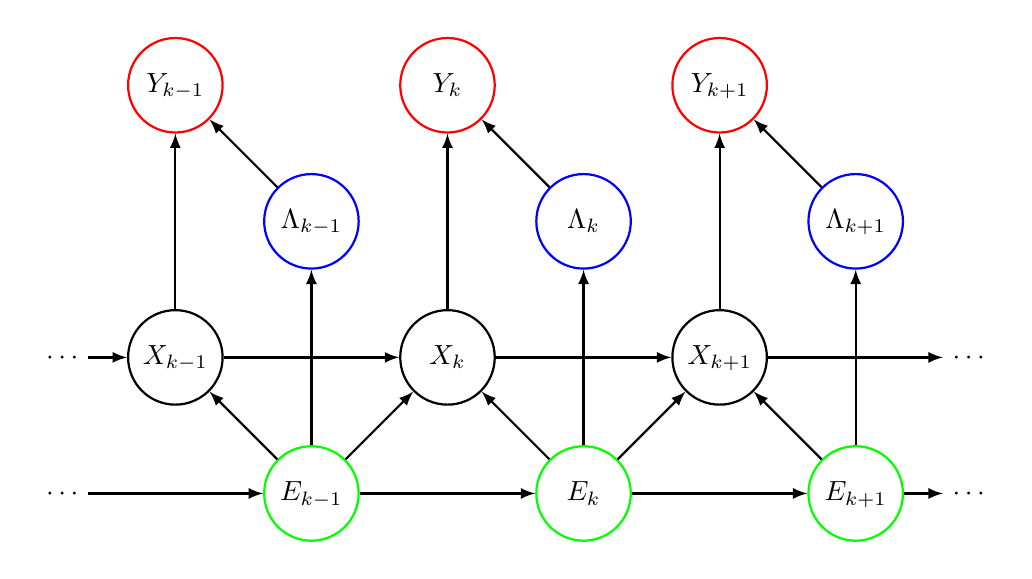
\begin{tikzpicture}[>=latex,text height=1.5ex,text depth=0.25ex]

	\matrix[row sep=0.5cm,column sep=0.5cm] {
		&
		\node (y_k-1) [observ]{$Y_{k-1}$}; &
		&
		\node (y_k) [observ]{$Y_{k}$}; &
		&
		\node (y_k+1) [observ]{$Y_{k+1}$}; &
		& \\
		& &
		\node (l_k-1) [assoc]{$\Lambda_{k-1}$}; &
		&
		\node (l_k) [assoc]{$\Lambda_{k}$}; &
		&
		\node (l_k+1) [assoc]{$\Lambda_{k+1}$}; & \\
		\node (x_k-2) {$\cdots$}; &
		\node (x_k-1) [state]{$X_{k-1}$}; &
		&
		\node (x_k) [state]{$X_{k}$}; &
		&
		\node (x_k+1) [state]{$X_{k+1}$}; &
		&
		\node (x_k+2) {$\cdots$}; \\
		\node (e_k-2) {$\cdots$}; & &
		\node (e_k-1) [exist]{$E_{k-1}$}; &
		&
		\node (e_k) [exist]{$E_{k}$}; &
		&
		\node (e_k+1) [exist]{$E_{k+1}$}; &
		\node (e_k+2) {$\cdots$}; \\
	};

	\path[->]
		(x_k-2) edge[thick] (x_k-1)
		(x_k-1) edge[thick] (x_k)
		(x_k) edge[thick] (x_k+1)
		(x_k+1) edge[thick] (x_k+2)
		
		(x_k-1) edge[thick] (y_k-1)
		(x_k) edge[thick] (y_k)
		(x_k+1) edge[thick] (y_k+1)
		
		(l_k-1) edge[thick] (y_k-1)
		(l_k) edge[thick] (y_k)
		(l_k+1) edge[thick] (y_k+1)
		
		(e_k-2) edge[thick] (e_k-1)
		(e_k-1) edge[thick] (e_k)
		(e_k) edge[thick] (e_k+1)
		(e_k+1) edge[thick] (e_k+2)
		
		(e_k-1) edge[thick] (x_k-1)
		(e_k) edge[thick] (x_k)
		(e_k+1) edge[thick] (x_k+1)
		
		(e_k-1) edge[thick] (x_k)
		(e_k) edge[thick] (x_k+1)
		
		(e_k-1) edge[thick] (l_k-1)
		(e_k) edge[thick] (l_k)
		(e_k+1) edge[thick] (l_k+1)
		;

\end{tikzpicture}
\caption{Graphical model for the modified target tracking model including target existence variables.}%
\label{fig:HMMExist}%
\end{figure}

Consider each of these terms. The form of the likelihood changes little.

\begin{multline}
P(Y_t|X_t, \Lambda_t, E_t) = V^{-(M_t-M_{T,t})} \prod_{\lambda_{j,t} \ne 0} P(y_t^{(\lambda_{j,t})}|x_{j,t}) \\
= V^{-(M_t-K_{\max})} \prod_{j=1}^{K_{\max}} \begin{cases} P(y_t^{(\lambda_{j,t})}|x_{j,t}) & e_{j,t} = 1, \lambda_{j,t} \ne 0 \\ V^{-1} & e_{j,t} = 0 \text{ or } \lambda_{j,t} = 0 \end{cases}
\label{eq:MTLikelihood}
\end{multline}

The association likelihood becomes:

\begin{equation}
P(\lambda_t|E_t) = \frac{\exp(-\mu_C) \mu_C^{(M_t-K_{\max})}}{M_t!} \prod_{j=1}^{K_{\max}} \begin{cases} P_D & e_{j,t} = 1, \lambda_{j,t} \ne 0, \lambda_{j,t} \notin \{ \lambda_{1:j-1,t} \} \\ 0 & e_{j,t} = 1, \lambda_{j,t} \in \{ \lambda_{1:j-1,t} \} \\ (1-P_D) \mu_C & e_{j,t} = 1, \lambda_{j,t}=0 \\ \mu_C & e_{j,t} = 0 \end{cases}
\label{eq:MTFactorisedAssociationLikelihoodWithE}
\end{equation}

The transition density becomes more complex. When targets appear we assume that their kinematic states are distributed according to some birth distribution $P_b(x_{j,t}$, known a priori. This may be uniform. Before targets have appeared and after they have died we set their state to some fixed dead-state. Thus we have

\begin{equation}
P(X_t|X_{t-1}, E_t, E_{t-1}) = \prod_{j=1}^{K_{\max}} \begin{cases} P(x_{j,t}|x_{j-1}) & e_{j,t} = 1, e_{j,t-1} = 1 \\ P_b(x_{j,t}) & e_{j,t} = 1, e_{j,t-1} = 0 \\ \delta_{x_{\text{dead}}}(x_{j,t}) & e_{j,t} = 0 \end{cases}
\label{eq:MTFactorisedTransitionWithE}
\end{equation}

Finally we need an expression for the existence transitions. We assume that targets have a fixed, independent probability of disappearing at any time, and that new targets are generated according to a Poisson process. Thus

\begin{equation}
P(E_t|E_{t-1}) = \frac{ \exp(\mu_{\text{birth}}) \mu_{\text{birth}}^{K_{\text{new},t}} }{ K_{\text{new},t} } \prod_{j=1}^{K_{\max}} \begin{cases} 1-P_{\text{death}} & e_{j,t} = 1, e_{j,t-1} = 1 \\ P_{\text{death}} & e_{j,t} = 0, e_{j,t-1} = 1 \end{cases}
\label{eq:MTExistenceTransition}
\end{equation}

where $K_{\text{new},t}$ is the number of targets present in frame $t$ which were not present in frame $t-1$.



\section{Particle filtering}
A particle filter for joint target detection and state estimation was implemented using a fixed lag SISR particle filter. Target disappearance requires only a trivial change, allowing the proposal that a track should end with some small probability.

Target appearance is a greater challenge, as the dimensionality of the state space expands enormously (any number of targets can appear in any location). In order to devise a practical algorithm, we use the method of a `search track' of \cite{Horridge2009}. The SISR particle filter already requires that we assume independence between targets. We assume that $\mu_{\text{birth}}$ is low enough that the probability of more than 1 track appearing at a given time is negligible. Then, we simply need one extra track whose particles represent the associations and states of a potential new target. When these search particles are observed to cluster in one location, we conclude that a new target has appeared and a new target filter is initiated.

A new mechanism is be required for proposing the observation associations for the search track particles, as we have no knowledge about the target position or velocity. Once the associations are proposed, the usual method for state proposals may be used. In even moderate clutter some scheme is needed to identify likely sites where a new target may have appeared, for example, by locating strings of observations in close proximity over time. These sites can be used to propose search particle associations. Without such a heuristic frontend, the probability of putting particles in the right place is likely to be very low.

An example of the SISR algorithm with lag 5 tracking 5 targets is shown in figure~\ref{fig:DetectionTracking}, using the linear-Gaussian observation model. Process and observation noises are set to 1, detection probability is 0.9 and expected number of clutter observations is 200 per frame.

\begin{figure} \centering
\subfigure[Observations]{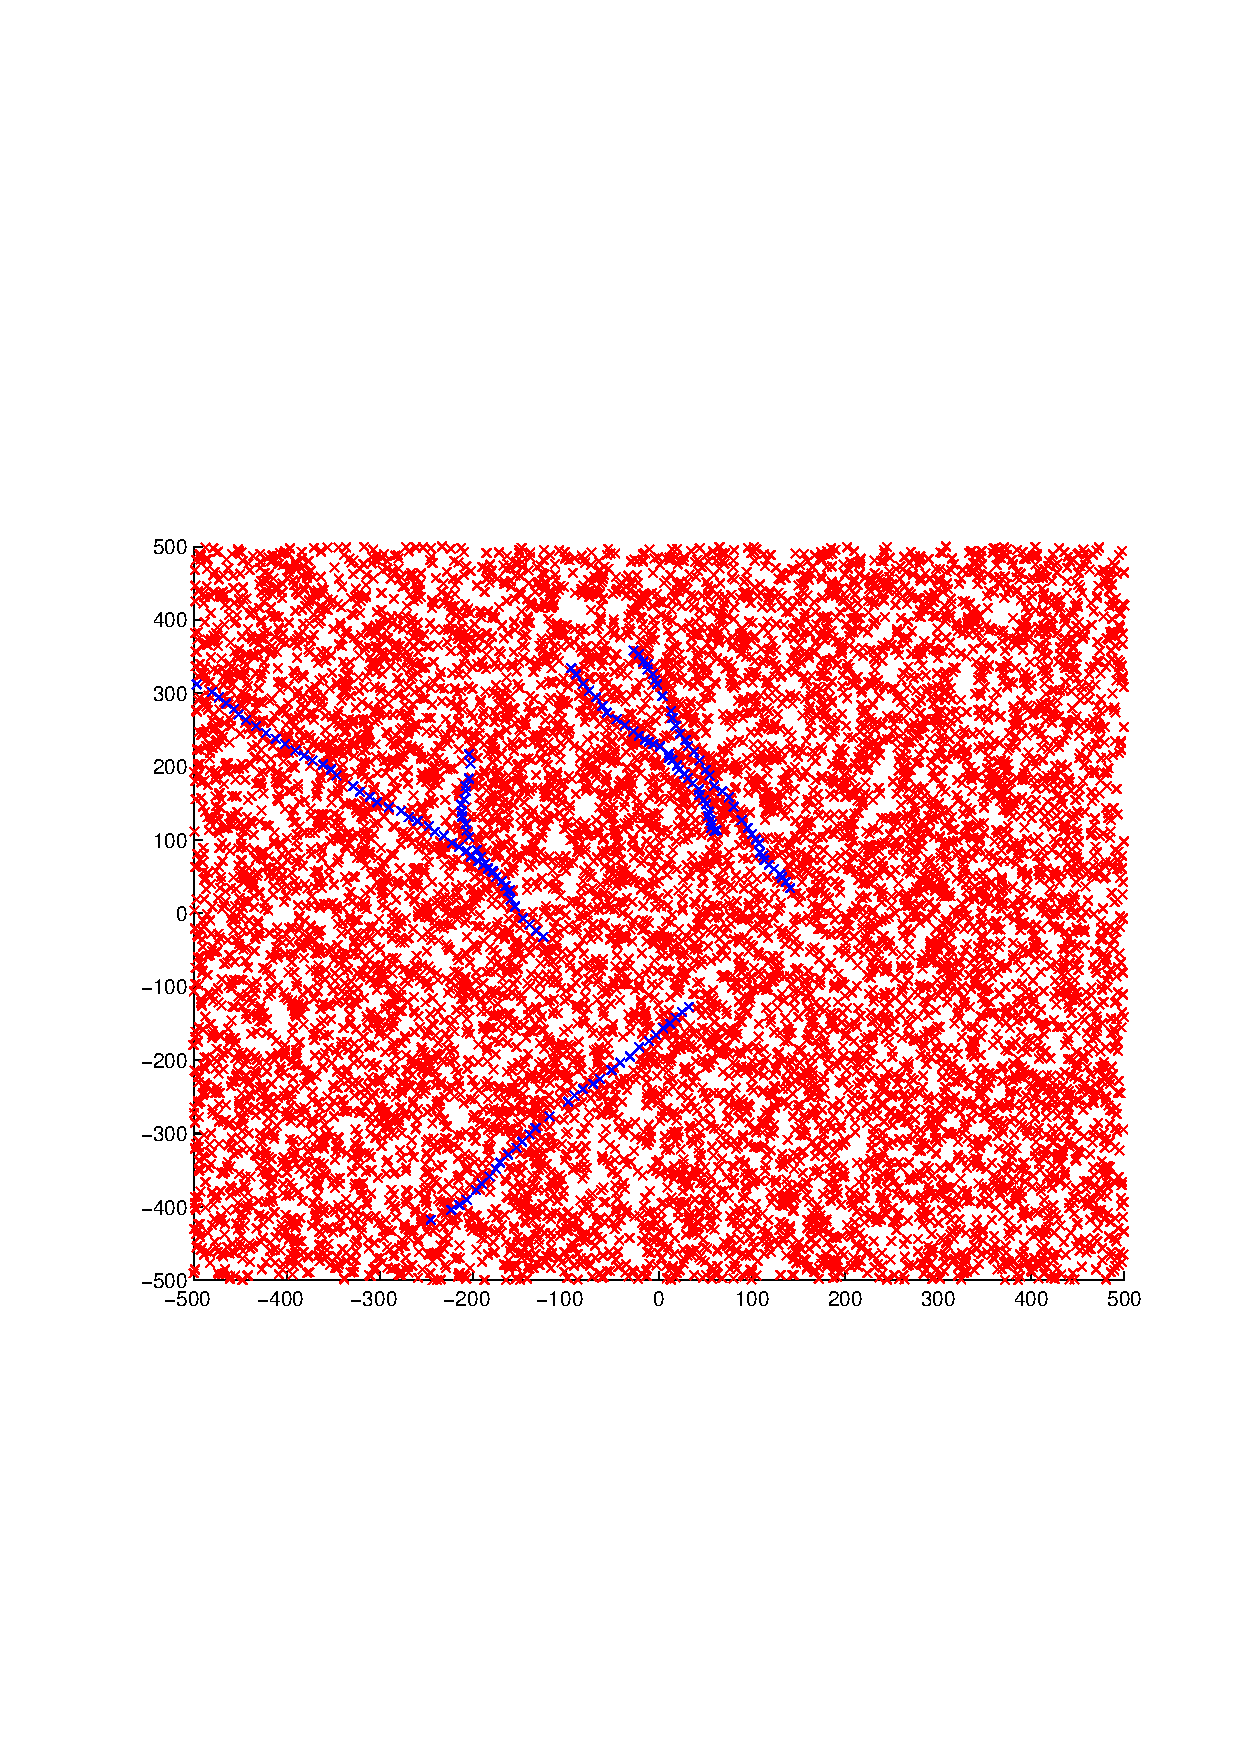
\includegraphics[width=0.45\columnwidth]{DetectionTrackingObs.pdf}}
\subfigure[States and Particle Estimates]{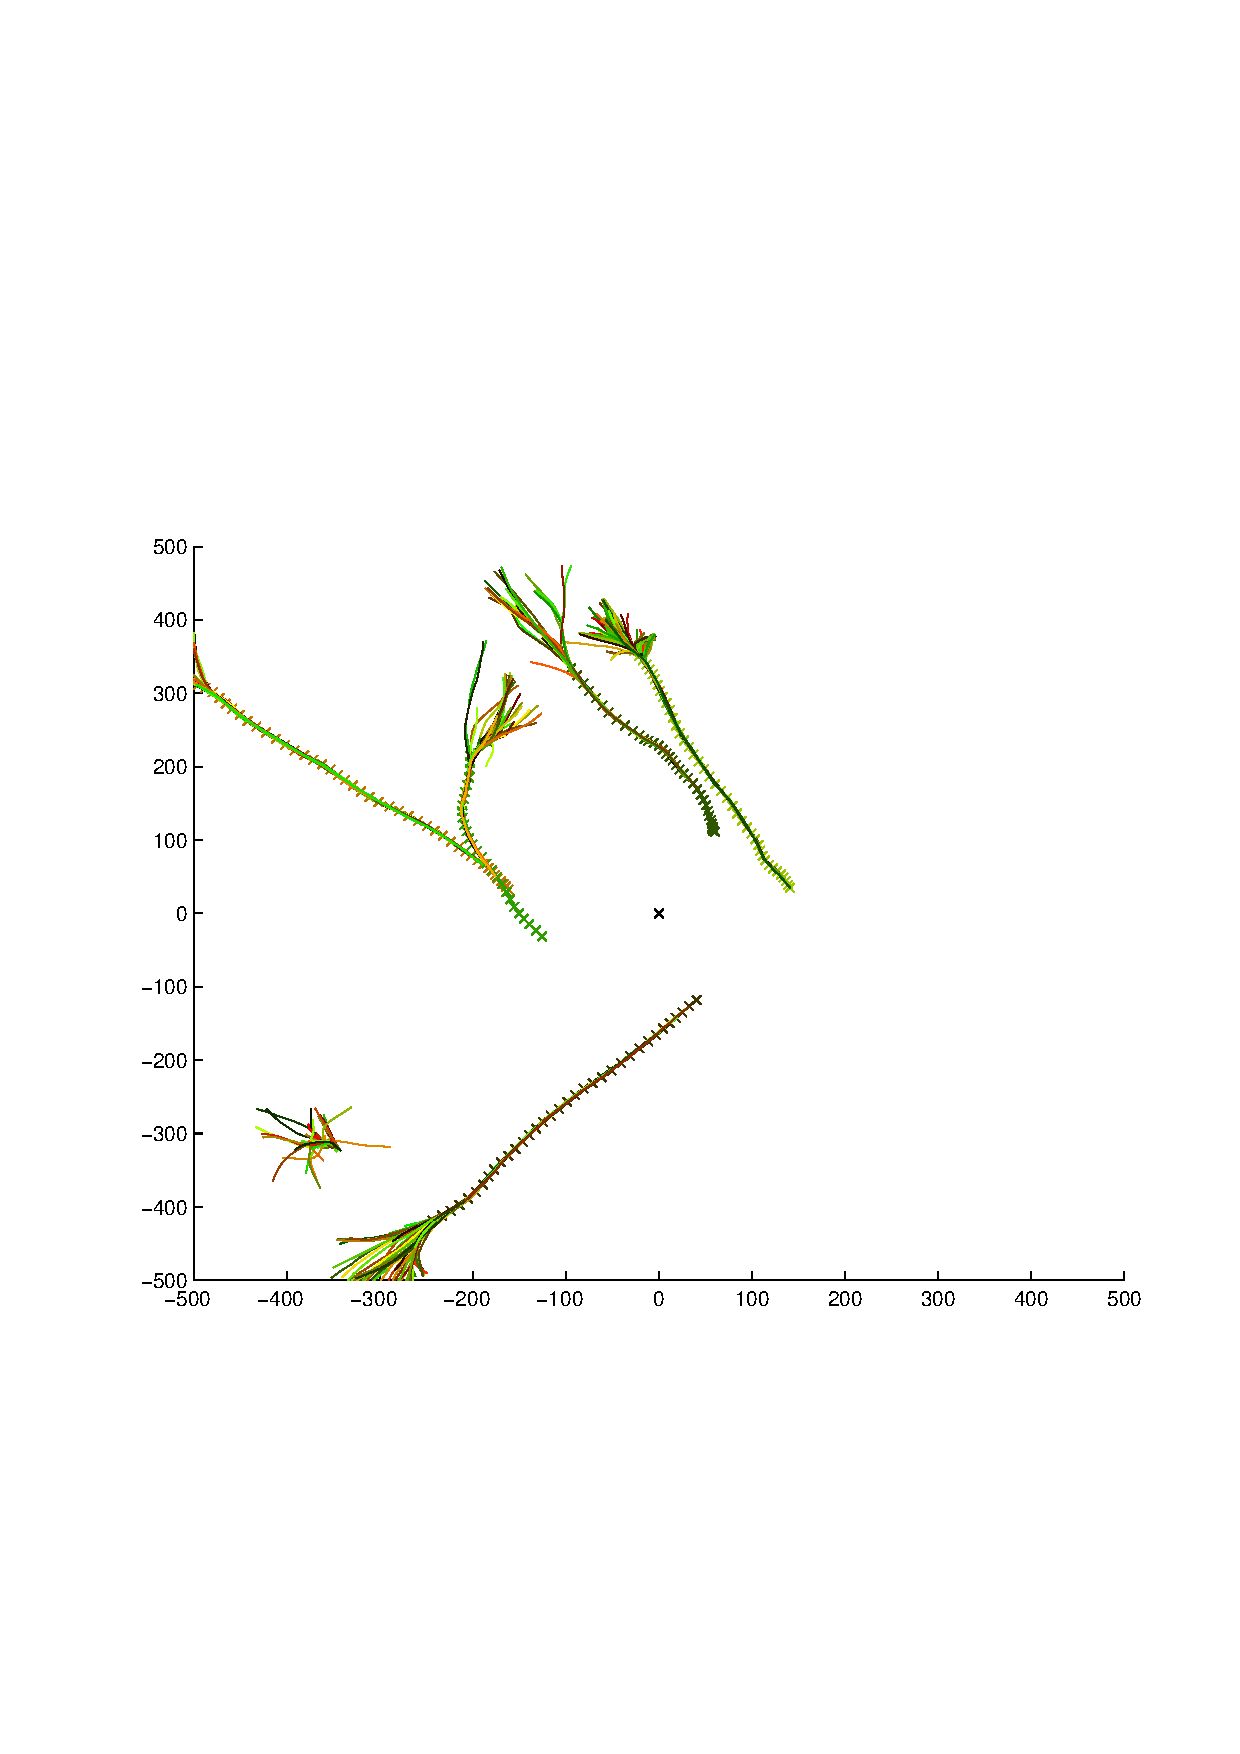
\includegraphics[width=0.45\columnwidth]{DetectionTracking.pdf}}
\caption{Target detection and tracking with fixed lag SISR algorithm with lag 5.}%
\label{fig:DetectionTracking}%
\end{figure}